\chapter{红外图像无人机目标检测相关理论}

\section{人工神经网络}
人工神经网络又称为类神经网络,一般简称神经网络。在机器学习领域中是一种模仿生物的神经网络结构的计算模型。这种模型常常被用来估计一种未知的函数。神经网络由大量的传输节点构成,这些传导节点也可以称为人工神经元。这些节点往往由若干个参数进行定义,这些参数就称为模型的权重。这些权重能够借助外界的信息对自身的值进行更新,也就是模型具备学习功能。在很多领域,神经网络能有类似人类的决定能力,因此很多传统编程方法难以解决的问题都可以用神经网络来进行解决。

一般意义上的神经网络主要由三个部分组成:结构、激活函数和学习规则。
结构主要指的是网络中的各种节点的计算方法和各节点之间的关系,一般指的是网络的权重。激活函数指的是将神经网络中某一层的计算结果进行某种的特定运算来扩大网络拟合结果的范围,提升网络对目标函数的拟合能力。学习规则指的是网络通过训练更新参数的具体策略。

\section{卷积神经网络}
卷积神经网络的主要特点是引入了卷积操作,通俗地说,卷积操作就是对输入的某个向量应用某种向量乘法,这种卷积操作对于提取某个区域的整体信息有较好的效果,因此在目标检测、图像分类、自然语言处理等计算机视觉任务中基于卷积神经网络的算法都能取得更好的性能。一般情况下卷积神经网络的主要组成如图\ref{cnn}所示,
卷积神经网络按照推理计算的顺序可以分为输入端、卷积层、池化层、全连接层等部分。

\begin{figure}[htbp]
    \centering
    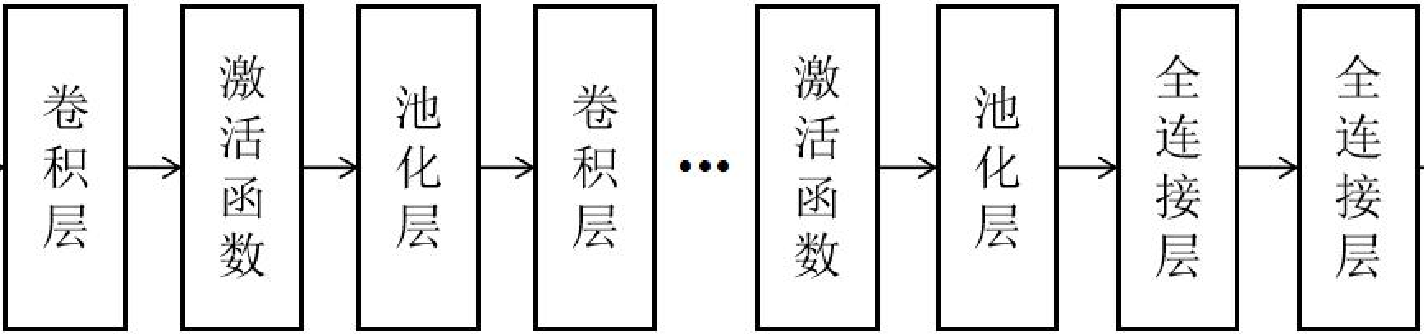
\includegraphics[width = 0.9\textwidth]{cnn.png}
    \caption{卷积神经网络常见结构}
    \label{cnn}
\end{figure}

下文将对卷积神经网络的各个主要组成部分进行介绍。

\subsection{卷积层}
卷积层的作用是定义一种卷积的运算方法。该层的权重参数经过训练后就用来对输入图像等张量进行特定的卷积运算,一般的作用是提取出重要特征。
通常卷积运算的公式可以写成如式\ref{conv1}所示:
\begin{equation}
    \mathrm{s}(t)=\left(x^{*} w\right)(t)
    \label{conv1}
\end{equation}

\begin{figure}[htbp]
    \centering
    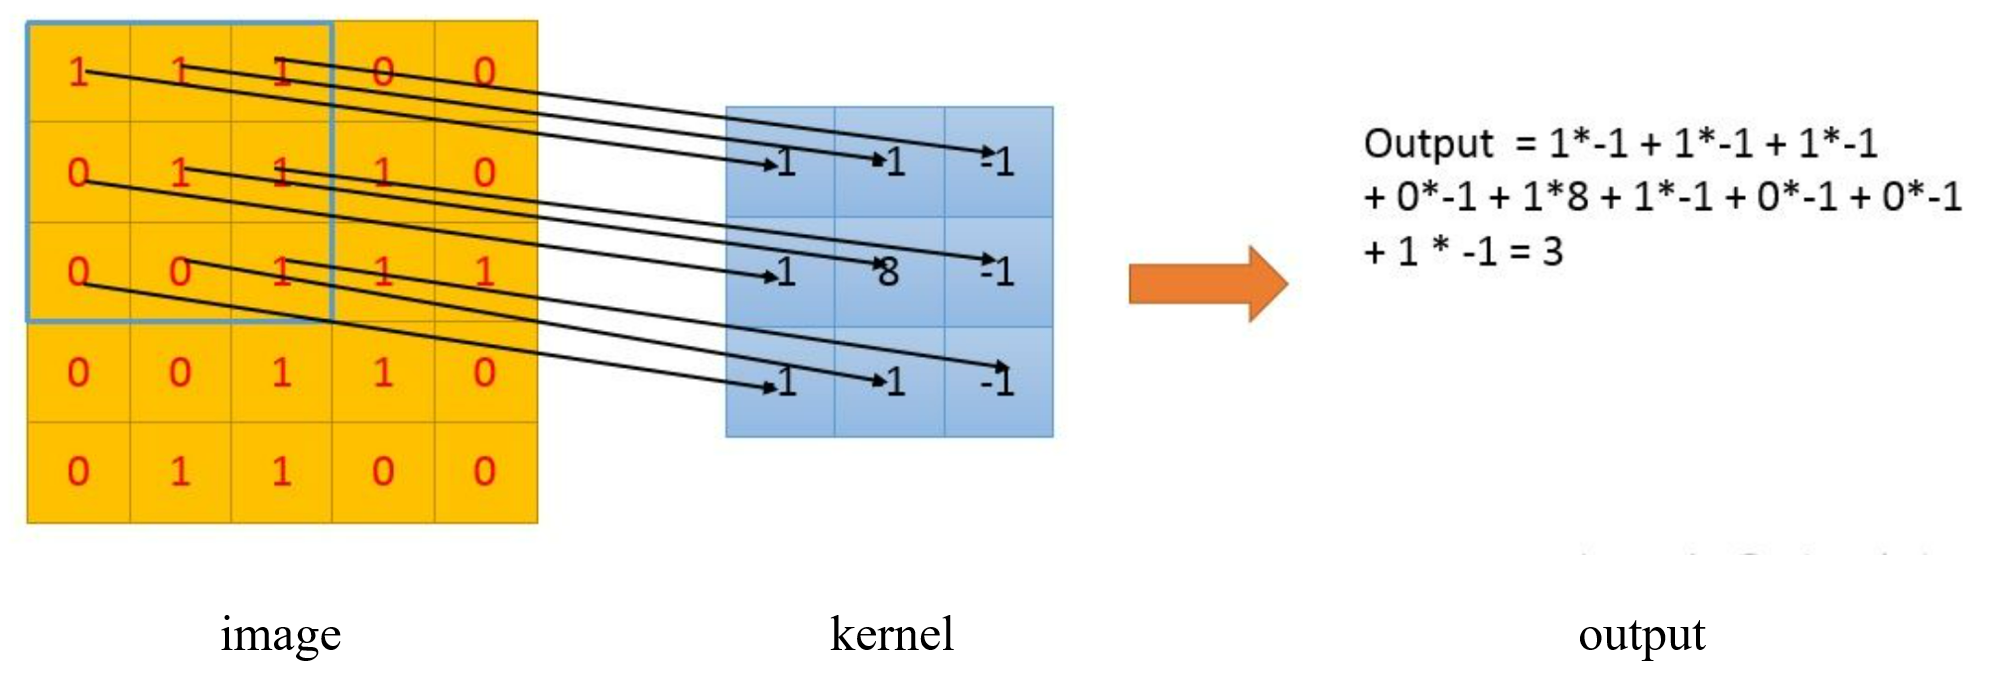
\includegraphics[width = 0.9\textwidth]{jjgc.png}
    \caption{图像卷积运算过程}
    \label{jjgc}
\end{figure}

式中$x$代表输入张量,$w$ 代表定义卷积核的函数。
对于在图像中的卷积运算,卷积核和输入图像之间的卷积运算可以视为矩阵乘法,因为卷积核的大小往往比输入图像小很多,卷积操作往往是一种提取图像局部特征的操作。
对图像的卷积过程如图\ref{jjgc}所示,
假设输入图像经过处理后可以视为$5\times5$的矩阵,卷积核的尺寸为
$3\times3$,卷积操作的具体过程就是从图像的左上角往右下角遍历,在每一次的遍历过程中将输入图像和卷积核进行比对,将输入图像和卷积核上对应位置的值进行相乘之后累加起来,每一次卷积核的运算对应一个运算结果,该运算结果是一个标量,并且根据卷积核的运算轨迹,该运算结果也将填在总体的卷积运算结果对应的输出矩阵的对应位置上。
卷积运算输出特征图的尺寸由式\ref{cout}决定,
\begin{equation}
    N_{\text {output }}=\frac{\left(W_{\text {input }}-F+2 P\right)}{S}+1
    \label{cout}
\end{equation}

式中,$W$代表输入图像的尺寸,$F$ 表示卷积核的尺寸, $P$ 表示 padding 填充的像素个数,$S$ 代表卷积核移动的步长。
通过训练,可以更新卷积核的参数,最理想的训练达到的效果是每个卷积核都完美地拟合到它们各自应该具备的功能上,比如提取目标的边缘、提取目标的某种形态等。这样整个卷积神经网络中的卷积核相互协作,共同完成整个系统应该具备的算法功能,并且取得较好的性能。卷积神经网络的核心思想就是通过训练使得网络中的各个卷积核具备最接近最佳算法的参数权重,从而达到拟合出处理输入对象的正确目标函数的目的。

\subsection{激活函数}
激活函数的主要作用是解决非线性问题。在神经网络的推理计算过程中,由于计算基本上由线性加权运算组成,因此运算的结果往往缺乏对非线性目标函数的拟合性能,这时就需要引入激活函数来增强网络的非线性。
常用的激活函数如下:

(1)Sigmoid 函数:Sigmoid函数也称Logistic 函数,是一种典型的激活函数,该函数的数学定义式可以写作如式\ref{log}所示,
\begin{equation}
    \sigma(x)=\frac{1}{\exp (-x)+1}
    \label{log}
\end{equation}

\begin{figure}[htbp]
    \centering
    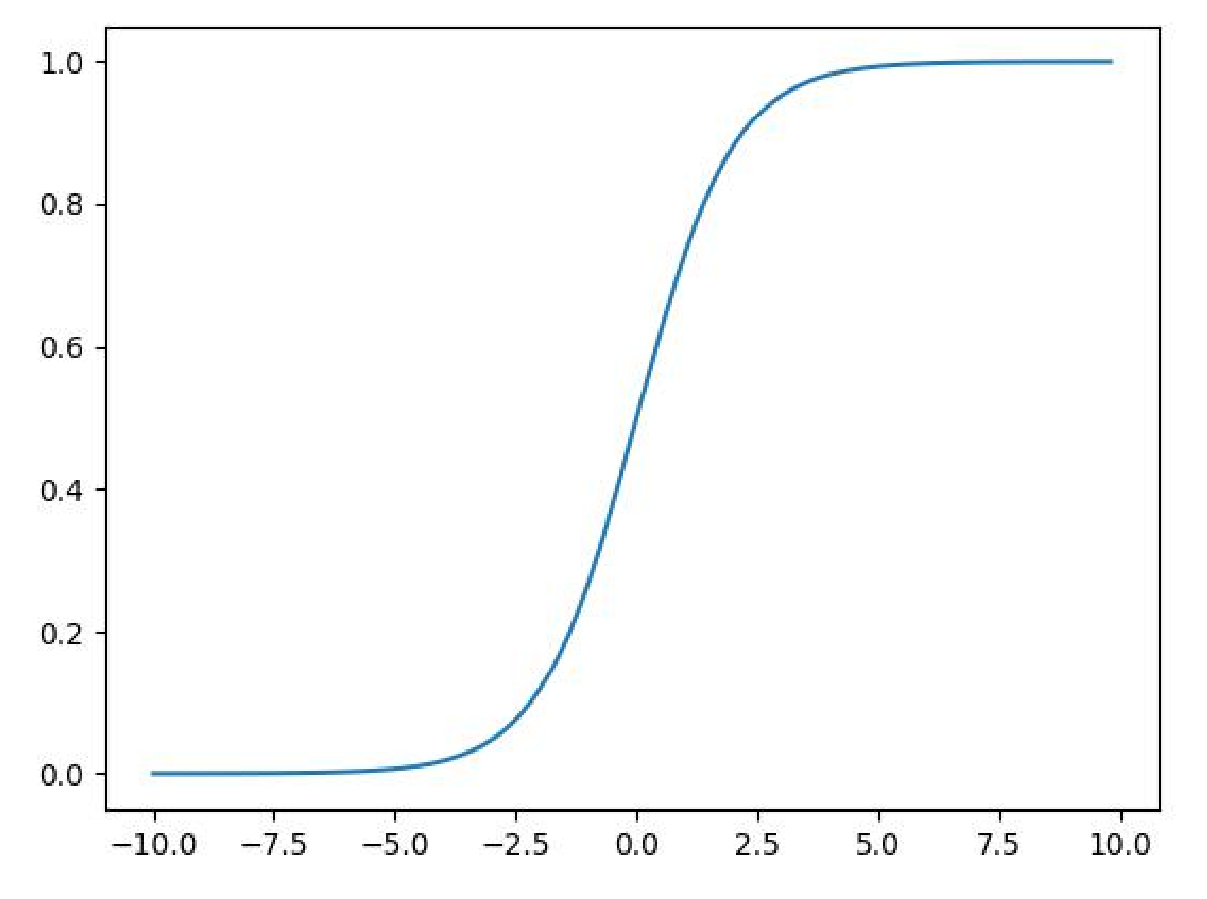
\includegraphics[width = 0.5\textwidth]{sigmoid.png}
    \caption{Sigmoid函数}
    \label{sig}
\end{figure}

\begin{figure}[htbp]
    \centering
    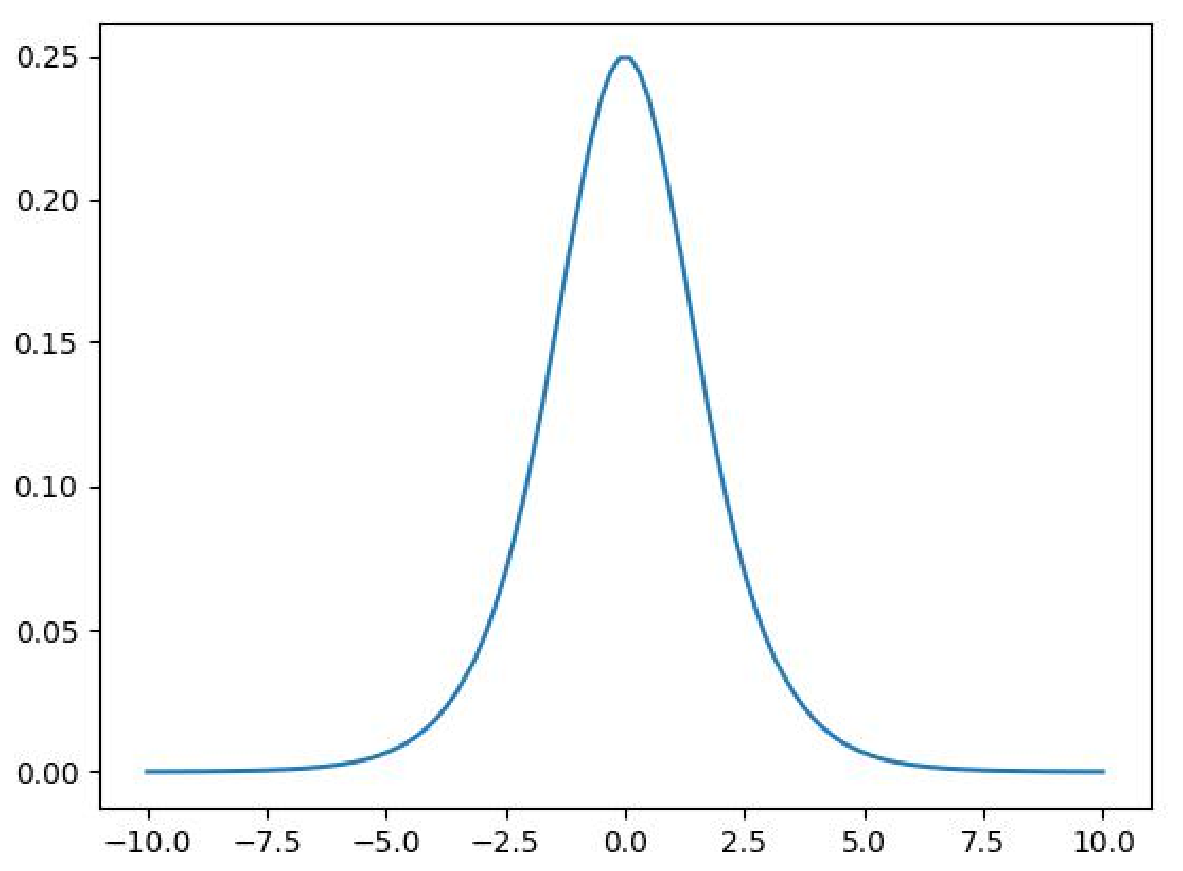
\includegraphics[width = 0.5\textwidth]{sig导数.png}
    \caption{Sigmoid导函数}
    \label{sigd}
\end{figure}

Sigmoid函数的图像如图\ref{sig}所示,由该图像可知,在输入Sigmoid函数系统处理后,输出的范围在$[0,1]$,因此该函数可以应用于二分类任务。Sigmoid函数的导数如图\ref{sigd}所示,从图中可知,
Sigmoid函数的微分容易计算,但是Sigmoid函数存在的问题是但输入不在特定范围内时会出现“梯度消失”的情况,影响模型的训练效果。针对这种梯度消失的问题,后续的研究人员提出了ReLU函数。

(2)Tanh 函数:Tanh 函数又叫做双曲正切激活函数,该函数的主要贡献是一定程度上解决了Sigmoid函数中存在的均值问题。Tanh函数的定义式如式\ref{tanh}所示,Tanh函数的图像如图\ref{tanh}所示,
由图\ref{tanh}可知,输入数据在经过Tanh函数的处理后输出范围是$[-1,1]$,并且该函数的图像在直角坐标系中是以原点为中心呈中心对称的,因此可以将Tanh函数视为Sigmoid函数经过平移和拉长的改进版本。虽然Tanh函数在实验中的性能相比Sigmoid函数有所提升,但是梯度消失的问题仍然存在。

\begin{equation}
    \sigma(x)=\tanh (x)=\frac{\exp (x)-\exp (-x)}{\exp (x)+\exp (-x)}=2 \operatorname{sigmoid}(2 x)-1
    \label{tan}
\end{equation}

\begin{figure}[htbp]
    \centering
    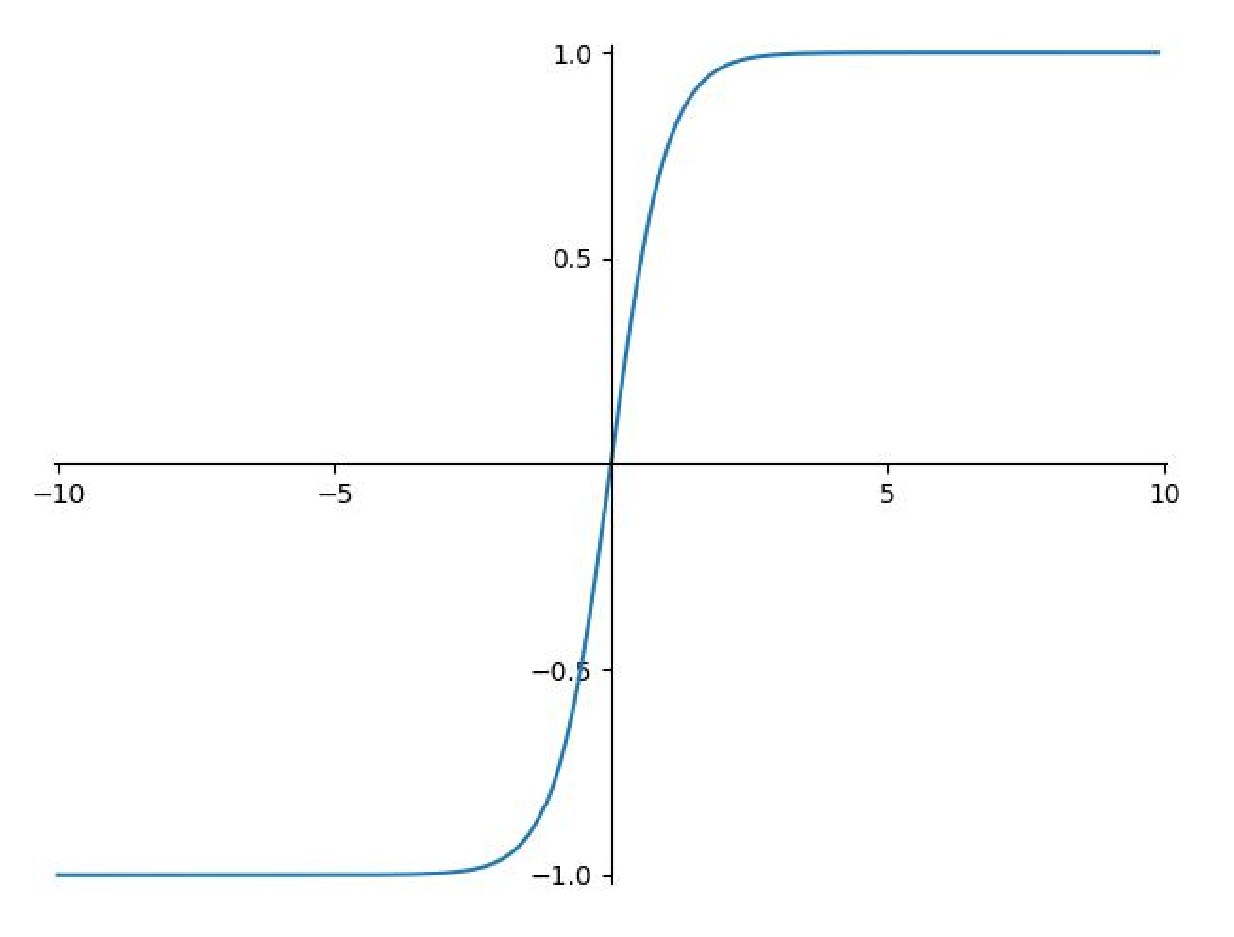
\includegraphics[width = 0.5\textwidth]{tanh.png}
    \caption{Tanh函数}
    \label{tanh}
\end{figure}

(3)ReLU 函数:ReLU函数的定义可以写作如式\ref{relu}所示,2010 年
Hinton 和 Nair 等人经过对神经网络结构的研究和分析,提出了ReLU函数。从ReLU函数的导函数中可知, ReLU 函数具备在$x\ge 0$时导数值为 $1$的特性,因此ReLU函数有对梯度消
失现象进行了有效的处理,这也使得ReLU函数成为了各类卷积神经网络中最常用的激活函数之一\cite{xu2015empirical}。ReLU函数和上文提到的Sigmoid函数和Tanh函数的主要区别是,该函数的定义式十分简单,在实际运算过程中也具备很快的计算速度。但ReLU函数的主要问题是将$ x<0$的部分
强制输出$0$,这中处理方法可能会导致“死区”问题,因此后续的研究人员提出了LeakyReLU\cite{maas2013rectifier}等改进版本。

\begin{equation}
    \sigma(x)=\max (0, x)= \begin{cases}x & x \geq 0 \\ 0 & x<0\end{cases}
    \label{relu}
\end{equation}

\subsection{池化层}
卷积网络的一个典型的模块组合方式是卷积、激活和池化。具体的流程是首先通过卷积层上的各个卷积核对输入特征图进行卷积运算,得到输出的特征图,在得到卷积产生的特征图后将结果输入激活函数中,将输出的特征进行激活处理,激发网络计算的非线性,最后一步就是池化操作,主要作用是将卷积和前序模块提取的特征进行合并和稀疏化,从而增强网络对整体特征的感知能力,同时减少网络的运算量。
最大池化运算的主要过程如图\ref{maxp}所示。
实际的卷积神经网络应用中,经常使用的池化方法主要有最大池化、平均池化等。
一般情况下,卷积神经网络池化层的主要功能可以归纳为以下几点:

(1)目标特征形态不变性。
由于池化过程一般是以某个区域内的某个点作为池化层的输出,所以即使该点在该区域中
产生了一定程度的位移,只要位移后的位置仍然位于该区域内,池化层输出的特征向量就不会受到影响,因此从具体意义上来看,图像上的某个特征点就算产生了一些位移,对于池化层来说这种位移是不对输出产生影响的。

(2)降低输出特征图的维度。
池化运算相当于对输入特征图以一定规则进行了缩小,得到的输出图像就是输入特征图的某些像素点重新拼接后组成的特征图,因此也称为降采样过程。

(3)池化层的处理导致的必然结果是降低整个模型的计算量和参数量,包括池化层后续的模块的参数量,因此也对解决过拟合问题有所贡献\cite{gu2018recent}。

\begin{figure}[htbp]
    \centering
    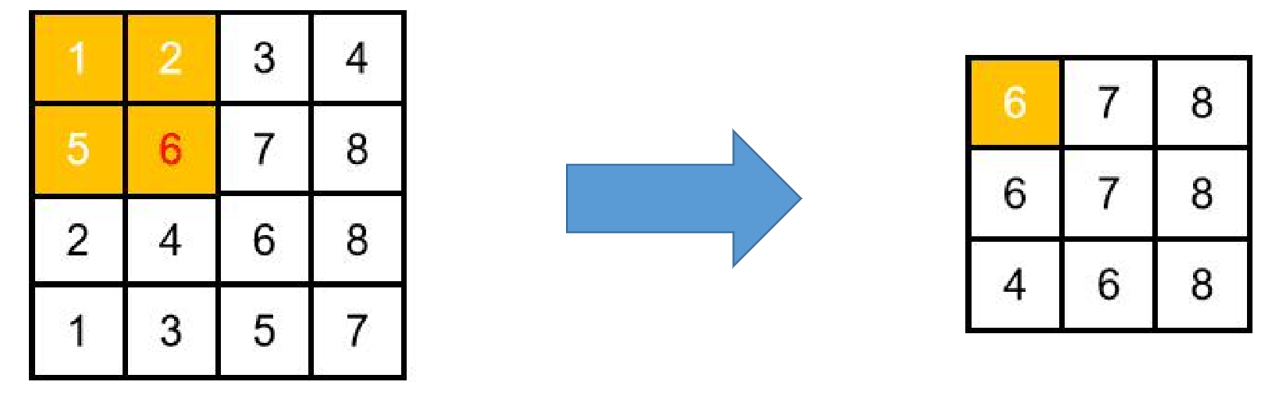
\includegraphics[width = 0.9\textwidth]{maxp.png}
    \caption{最大池化示意图}
    \label{maxp}
\end{figure}

\subsection{全连接层}
全连接层在经典的全连接网络中比较常见,在卷积神经网络中,通常采用少量的全连接层,对前序的卷积层等模块所提取出的图像目标特征等信息进行整合和判决,从而输出整个算法的最终结果。但是全连接层一般接收的输入张量大小是固定不变的,所以实际算法应用中往往采用卷积层来替代全连接层,组成全卷积网络,用卷积层进行网络的输出同样可以起到整合结果、得出结论的作用。

\section{目标检测的评价指标}
在绝大多数研究中,目标检测算法的性能通常可以由两个指标来进行衡量和比较,即
平均准确度均值(the mean
Average Precision,mAP)
和FPS(Frames per second)。

mAP主要由两个方面组成,分别是模型的精确率(Precision)和召回率(Recall)。通俗地说,优秀的目标检测精度就是指精确率和召回率都能处在较高水平。平均准确度就是指综合考虑精确率和召回率之后得出的性能表现,而均值指的是目标检测中每个待测目标类型都会得出一个平均准确度,平均准确度均值就是将这若干个平均准确度进行算术平均后得到的值。AP(Average-Precision)的具体计算方法是根据取不同的置信概率阈值得到的召回率和精确率的值同时在一个直角坐标系内描点,在连线后求该曲线和坐标系包围的区域的面积。直观地,对每个固定地置信概率值,精确率和召回率都较高的模型能获得更高的AP值。
下面介绍与 AP 相关指标的概念。

(1)IoU:衡量模型计算得出的预测框和真值框之间的匹配程度的一种标准,主要计算方法是将预测框和真值框的相交部分面积和这两个部分的相并区域面积作比,如果IoU值较高,就认为模型对目标的定位能力较强,对于检测任务来说,一次成功的检测往往要求预测框和真值框的IoU大于某个标准,如$0.5$等。

(2)True和False、Positive和Negative:True或是False指的是模型得出的判断对照真值后可知是正确的判断或是错误的判断,而Positive或是Negative指的是模型算法对某个区域的计算结果是认为该区域有某种类型的目标,或是模型不认为该区域有某种类型的目标。具体地,True Positive指的是模型对该区域做出的判断是有某种类型的目标,而经过和真值框的对照,该区域确实存在该类型的目标,模型的判断结果正确。True Negative是指模型的判断是该区域不存在某类型目标,真值中确实也不存在该类型目标,模型的判断结果正确。False Positive指的是模型的判断结果是该区域存在某类型目标,但是真值中该区域不存在该类型目标,模型判断错误。False Negative是指模型判断该区域存在某类型目标,但是真值中存在该类型目标,因此模型判断错误。
在计算量化时,通常将TP、TN、FP、FN表示成符合上述情况的示例的数量。

(3)精确率:精确率的定义式如
式\ref{pr}所示。精确率表示模型判断出存在的目标数量且验证未正确的数量占模型判断出的所有目标的比例,衡量的是模型做出的判断中有多少是准确的。

\begin{equation}
     \text { Precision }=\frac{T P}{T P+F P}
    \label{pr}
\end{equation}

(4)召回率:召回率的定义式如
式\ref{rec}所示。召回率表示模型判断出的目标数量和真值中总共存在的所有目标数量的比值,表示真值中的样本有多少被模型计算找出,衡量模型对目标的发现能力。

\begin{equation}
     \text { Recall }=\frac{T P}{T P+F N}
    \label{rec}
\end{equation}

根据 Precision 和 Recall 的计算公式很容易得 Precision-Recall 曲线进而获得
AP 值,但不同的数据集计算 AP 值主要的区别在于 IoU 阈值的设定。对于 VOC
2007 来说 IoU 的阈值为 0.5,MS COCO 的 IoU 的阈值在[0.5,0.95]区间以 0.05 为
间隔设置多个阈值并且为了评价模型对不同大小目标的检测效果分别计算了大
中小型目标的 AP 值,ImageNet 的 IoU 阈值的设定与真值框的大小有关。

FPS(Frame Per Second),指的是模型每秒钟能够处理的图片数量。在实际
项目中除了需要有较高的检测精度外还需要很快的检测速度来实现实时检测的
目的,例如拿检测效果比较好的双阶段算法 Faster R-CNN 来说,每秒只能处理
几张图片,根本无法保证实时检测。而单阶段算法 YOLOv3 却能够每秒处理几
十张图片,这也是后面单阶段算法在项目中应用广泛的原因。

\section{红外成像原理}
传统上,红外技术与控制功能和夜视问题有关,早期的应用仅与探测红外辐射相联系,后来通过形成红外图像
,形成温度和发射率差异\cite{rogalski2002infrared}。现代红外技术的起源于第二次世界大战期间。最近在将红外技术应用于遥感问题方面取得的成功是由于近50多年来对高性能红外探测器的成功开发。大部分资金已用于满足军事需要,但民用应用不断增加,特别是在20世纪的最后10年。这些应用包括医疗、工业、地球资源和节能应用。医学应用包括热成像,其中人体的红外扫描可以用于检测癌症或其他提高体表温度的创伤
。此外,地球上各种资源的确定可以通过使用来自卫星的红外图像与现场观察的校准。在某些情况下,甚至一种作物的健康状况也可以从太空中借助红外探测得到确定。利用红外扫描来确定最大热损失点,帮助了家庭和工业的节能。由于这些技术的有效应用,在全球环境污染和气候变化监测、农业作物产量的长期预测、化学过程监测、傅里叶变换红外光谱学、红外天文学、汽车驾驶、医学诊断中的红外成像等方面,使用这些技术的需求正在迅速增长。

红外目标检测可以分为图像预处理和目标检测两个步骤,因此在进行后续工
作前需要分析红外图像的获取过程以及红外图像存在的特性。本节从红外成像的理论基础、红外成像的过程、红外图像的特性等方面进行相关概念的介绍,为后续工作开展打下理
论基础。
\subsection{物体的热辐射}
红外成像和探测的基础是物体的热辐射。所有的物体都是由不断振动的原子组成的,能量较高的原子振动更频繁。所有带电粒子的振动,包括这些原子,都会产生电磁波。一个物体的温度越高,振动就越快,因此光谱辐射能就越高。因此,所有的物体都在不断地发射辐射,其波长分布取决于物体的温度及其光谱发射率。辐射发射通常用黑体的概念来处理。黑体是一个吸收所有入射辐射的物体,相反地,根据基尔霍夫定律,它是一个完美的辐射器。黑体发出的能量在理论上是在给定温度下可能达到的最大能量。辐射功率(或发射的光子数)及其波长分布可以由普朗克辐射定律给出,如式\ref{plank1}和式\ref{plank2}所示。
\begin{equation}
    W(\lambda, T)=\frac{2 \pi h c^{2}}{\lambda^{5}}\left[\exp \left(\frac{h c}{\lambda k T}\right)-1\right]^{-1} \quad \mathrm{~W} /\left(\mathrm{cm}^{2} \mu \mathrm{m}\right)
    \label{plank1}
\end{equation}

\begin{equation}
    P(\lambda, T)=\frac{2 \pi c}{\lambda^{4}}\left[\exp \left(\frac{h c}{\lambda k T}\right)-1\right]^{-1} \text { photons } /\left(\mathrm{s} \mathrm{cm}^{2} \mu \mathrm{m}\right)
    \label{plank2}    
\end{equation}

其中$\lambda$是波长,$T$是温度,$h$是普朗克常数,$c$是光速,$k$是玻尔兹曼常数。

\subsection{探测器}
红外探测器技术的研究进展主要与半导体红外探测器有关。在光子探测器中,辐射通过与电子的相互作用被材料吸收。观测到的电输出信号是由电子能量分布的变化引起的结果。光子探测器显示出每单位入射辐射功率响应的选择性波长。光子探测器能表现出完美的信噪比性能和非常快速的响应。但要实现这一点
,光子探测器需要低温冷却。冷却要求是基于半导体光电探测器的红外系统更广泛使用的主要障碍,使其体积大、重量大、昂贵并且
使用起来很不方便。根据相互作用的性质,光子探测器的类别被进一步细分为不同的类型。最重要的是:固有探测器、外在探测器、光发射探测器和量子阱探测器。
第二类红外探测器是由热探测器组成的。在热探测器中,入射辐射被吸收来改变材料的温度,而由此产生的某些物理性质的变化被用来产生电输出。探测器元件悬挂在与散热器上。热效应通常与波长无关;信号取决于辐射功率(或其变化率),而不是它的光谱含量。在热释电探测器中,测量内部自发极化的变化,而在测辐射热计的情况下,测量电阻的变化。与光子探测器相比,热探测器通常在室温下工作。它们通常的特点是中等灵敏度和反应缓慢
,但它们便宜和易于使用。

\subsection{红外成像过程}
红外线(IR)是波长在 760nm 到 1mm 之间,波长介于可见光与微波之间的
电磁波,自然界中任何物体只要温度在绝对零度($-273 ^{\circ}C$)以上都会产生红外
辐射。红外成像技术就是使用红外探测器接收物体发出的红外辐射,最后以红外
图像或视频等方式呈现出来。红外成像技术原理如图\ref{infra}所示\cite{倪国强2008中国红外成像技术发展的若干思考}。

\begin{figure}[htbp]
    \centering
    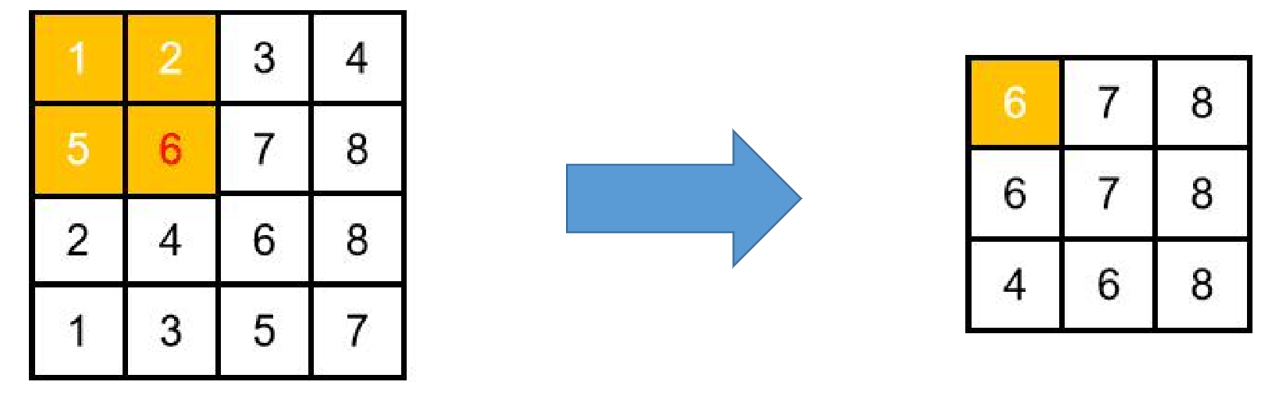
\includegraphics[width = 0.9\textwidth]{maxp.png}
    \caption{最大池化示意图}
    \label{infra}
\end{figure}

图\ref{infra}中展示了整个红外成像的过程,首先经过红外摄像机进行图像采集,由于
红外探测器性能及成本因素,将采集到的模拟信号首先进行模数转换,然后进行
图像处理,最后进行图像的展示或进行目标检测等后续工作。

\subsection{红外图像特性} 
根据红外成像技术原理,结合红外探测器性能的限制以及环境因素,导致红
外图像相比于可见光图像主要有以下特征:

(1)图像分辨率差、对比度低。由于红外图像是吸收红外辐射进行成像的,
而物体的红外辐射在传输过程中经过大气吸收以及环境散射等因素导致红外探
测器接收到的红外辐射会减少,就会导致成像对比度低。

(2)图像信噪比低。红外图像往往会存在着大量的噪声,一部分噪声来自
于设备噪声,由于红外探测器硬件原因会产生热噪声、三粒噪声、光子噪声等。
另一部分来自于环境噪声,这部分因素无法控制。

(3)物体边缘模糊。由于物体之间的热辐射可以相互影响,因此采集到的
图像会出现物体边缘没有明显的界限,这会对后续进行目标检测造成困难。

\section{本章小结}
本章主要介绍了基于深度学习的目标检测算法相关的一些理论基础以及简
要的介绍了红外图像的获取过程。首先对卷积神经网络的组成,包括卷积层、池
化层、全连接层以及激活函数做了详细的介绍,这些都是后续目标检测算法的重
要组成部件。然后介绍了基于深度学习的目标检测算法的性能评价指标以及指标
的计算过程。最后介绍了红外图像相关的知识。简单的概述了红外图像的获取过
程以及红外图像的特性,为后续进行红外图像预处理和网络结构的改进打下理论
基础。
